\documentclass{beamer}

\usetheme{Warsaw}

%\usetheme{Singapore}
%%% اینها هنوز کار نمی‌کنند.
%%\usetheme{Bergen}
%%\usetheme{AnnArbor}
%%\usetheme{CambridgeUS}
%%\usetheme{Hannover}
%%%\usetheme{Boadilla}
%%%\usetheme{Madrid}
%%%\usetheme{Antibes}
%%%\usetheme{Copenhagen}\setbeamercovered{dynamic}
%%% \usetheme{Marburg} 

\usefonttheme{serif}

\addtobeamertemplate{navigation symbols}{}{%
	\usebeamerfont{footline}%
	\usebeamercolor[fg]{footline}%
	\hspace{1em}%
	\insertframenumber/\inserttotalframenumber
}
\setbeamercolor{footline}{fg=blue}



\usepackage{graphicx}
\usepackage{ptext}
\usepackage{multicol}
\usepackage{xepersian}
\settextfont{Yas.ttf}
\setcounter{tocdepth}{1}


%%%%%%%%%%%%%%%%
%%%اینها تصحیحاتی لازمه کار هستند که توسط دکتر وفا خلیقی در پست‌های زیر نوشته شده است.
%%%http://qa.parsilatex.com/14100/
%%%http://qa.parsilatex.com/14148
%%%%%%%%%%شروع
%%% تصحیح دستورات \frametitle و \framesubtitle برای قرار دادن عنوان و زیرعنوان یک frame استفاده کنیم:
\makeatletter
\define@key{beamercolbox}{left}[0pt]{\def\beamer@colbox@rs{0pt}\def\beamer@colbox@ls{#1 plus1fill}}
\makeatother
%%% تصحیح محیط‌های لیست 
\makeatletter
\expandafter\let\csname beamer@@tmpop@itemize item@default\endcsname\relax
\expandafter\let\csname beamer@@tmpop@itemize subitem@default\endcsname\relax
\expandafter\let\csname beamer@@tmpop@itemize subsubitem@default\endcsname\relax

\defbeamertemplate*{itemize item}{default}{\scriptsize\raise1.25pt\hbox{\donotcoloroutermaths$\blacktriangleleft$}}
\defbeamertemplate*{itemize subitem}{default}{\tiny\raise1.5pt\hbox{\donotcoloroutermaths$\blacktriangleleft$}}
\defbeamertemplate*{itemize subsubitem}{default}{\tiny\raise1.5pt\hbox{\donotcoloroutermaths$\blacktriangleleft$}}

\bidi@patchcmd{\@listi}{\leftmargin}{\rightmargin}{}{}
\let\@listI\@listi
\bidi@patchcmd{\@listii}{\leftmargin}{\rightmargin}{}{}
\bidi@patchcmd{\@listiii}{\leftmargin}{\rightmargin}{}{}
\bidi@patchcmd{\beamer@enum@}{\raggedright}{\raggedleft}{}{}
\bidi@patchcmd{\@@description}{\raggedright}{\raggedleft}{}{}
\bidi@patchcmd{\@@description}{\leftmargin}{\rightmargin}{}{}

\renewcommand{\itemize}[1][]{%
  \beamer@ifempty{#1}{}{\def\beamer@defaultospec{#1}}%
  \ifnum \@itemdepth >2\relax\@toodeep\else
    \advance\@itemdepth\@ne
    \beamer@computepref\@itemdepth% sets \beameritemnestingprefix
    \usebeamerfont{itemize/enumerate \beameritemnestingprefix body}%
    \usebeamercolor[fg]{itemize/enumerate \beameritemnestingprefix body}%
    \usebeamertemplate{itemize/enumerate \beameritemnestingprefix body begin}%
    \list
      {\usebeamertemplate{itemize \beameritemnestingprefix item}}
      {\def\makelabel##1{%
          {%
            \hss\llap{{%
                \usebeamerfont*{itemize \beameritemnestingprefix item}%
                \usebeamercolor[fg]{itemize \beameritemnestingprefix item}##1}}%
          }%
        }%
      }
  \fi%
  \beamer@cramped%
  \raggedleft%
  \beamer@firstlineitemizeunskip%
}
\makeatother
%%%%%%%%%%%%%%%%%%%%%%%%%%%%%%%%%%%%%%


%%% تصحیح مشکل پانویس foornote

\makeatletter
\bidi@undef\beamer@@tmpop@footnote@default

\defbeamertemplate*{footnote}{default}
{
  \parindent 1em\noindent%
  \raggedleft
  \hbox to 1.8em{\hfil\insertfootnotemark}\insertfootnotetext\par%
}

\defbeamertemplate*{LTRfootnote}{default}
{
  \parindent 1em\noindent%
  \raggedright
  \hbox to 1.8em{\hfil\insertfootnotemark}\latinfont\insertfootnotetext\par%
}
\footdir@temp\footdir@ORG@bidi@beamer@framefootnotetext\beamer@framefootnotetext{R}
\let\@footnotetext=\beamer@framefootnotetext
\let\@RTLfootnotetext\@footnotetext

\def\@makeLTRfntext#1{%
  \def\insertfootnotetext{#1}%
  \def\insertfootnotemark{\@makefnmark}%
  \usebeamertemplate***{LTRfootnote}}

\newcommand<>\beamer@frameLTRfootnotetext[1]{%
  \global\setbox\beamer@footins\vbox{\@RTLfalse%
    \hsize\framewidth
    \textwidth\hsize
    \columnwidth\hsize
    \unvbox\beamer@footins
    \reset@font\footnotesize
    \@parboxrestore
    \protected@edef\@currentlabel
         {\csname p@footnote\endcsname\@thefnmark}%
    \color@begingroup
      \uncover#2{\@makeLTRfntext{%
        \rule\z@\footnotesep\ignorespaces#1\@finalstrut\strutbox}}%
    \color@endgroup}}


\footdir@temp\footdir@ORG@bidi@beamer@frameLTRfootnotetext\beamer@frameLTRfootnotetext{L}
\let\@LTRfootnotetext=\beamer@frameLTRfootnotetext

\makeatother

%%%%%%%%%%%%%%%%%%%%%%%%%%%%%%%%%%%




%%%تصحیح چپ‌چین شدن متن
\raggedleft

%%%%%%%%%%%%%%%%%%%%%%%%%%


%%%تصحیح محیط‌های قضیه، مثال و ....

\makeatletter
\renewenvironment{beamercolorbox}[2][]{%
  \begingroup%
    \def\beamer@colbox@coladd{0pt}%
    \def\beamer@vmode{\leavevmode}%
    \setkeys{beamercolbox}{%
      wd=\textwidth,ht={},dp={},%
      rightskip=0pt,leftskip=0pt plus1fil,%
      sep=0pt,colsep=0pt,colsep*=0pt,%
      shadow=false,rounded=false,ignorebg=false}%
    \setkeys{beamercolbox}{#1}%
    \ifbeamercolorempty[bg]{#2}{\@tempswafalse}{\@tempswatrue}%
    \ifbeamer@colbox@ignorebg\@tempswafalse\fi%
    \def\beamer@colbox@color{#2}%
    \hsize=\beamer@colbox@wd%
    \setbox\beamer@tempbox=\hbox\bgroup\vbox\bgroup%
      \leftskip=\beamer@colbox@ls%
      \advance\leftskip by\beamer@colbox@sep%
      \rightskip=\beamer@colbox@rs%
      \advance\rightskip by\beamer@colbox@sep%
      \ifbeamer@colbox@ignorebg%
        \colorlet{beamer@temp@color}{bg}%
        \usebeamercolor[fg]{#2}%
        \colorlet{bg}{beamer@temp@color}%
      \else%
        \usebeamercolor[fg]{#2}%
      \fi%
      \if@tempswa%
        \advance\leftskip by\beamer@colbox@colsep%
        \advance\rightskip by\beamer@colbox@colsep%
        \ifdim\beamer@colbox@colsep=0pt\else\vskip\beamer@colbox@colsep\fi%
        \ifdim\beamer@colbox@colseps=0pt\else\vskip\beamer@colbox@colseps\fi%
      \fi%
      \ifdim\beamer@colbox@sep=0pt\else\vskip\beamer@colbox@sep\fi%
      \beamer@vmode\ignorespaces}{%
      \ifdim\beamer@colbox@sep=0pt\else\vskip\beamer@colbox@sep\fi%
      \if@tempswa\ifdim\beamer@colbox@colsep=0pt\else\vskip\beamer@colbox@colsep\fi\fi%
      \if@tempswa\ifdim\beamer@colbox@colseps=0pt\else\vskip\beamer@colbox@colseps\fi\fi%
    \egroup\egroup%
    \wd\beamer@tempbox=\hsize%
    \@tempdima=\wd\beamer@tempbox%
    \ifx\beamer@colbox@ht\@empty%
    \else%
      \ht\beamer@tempbox=\beamer@colbox@ht%
    \fi%
    \ifx\beamer@colbox@dp\@empty%
    \else%
      \dp\beamer@tempbox=\beamer@colbox@dp%
    \fi%
    \ifbeamer@colbox@rounded%
      \if@tempswa%
        \begin{beamerboxesrounded}[%
          shadow=\beamer@colbox@shadow,%
          lower=\beamer@colbox@color,%
          upper=normal text,%
          width=\beamer@colbox@wd]{}%
          \box\beamer@tempbox%
        \end{beamerboxesrounded}%
      \else%
        \ifdim\@tempdima>\textwidth%
          \setbox\beamer@tempbox=\hbox to\textwidth{\hss\box\beamer@tempbox\hss}%
        \fi%
        \box\beamer@tempbox%
      \fi%
    \else%
      \if@tempswa\setbox\beamer@tempbox=\hbox{\vbox{%
        \usebeamercolor{\beamer@colbox@color}%
        \advance\hsize by \beamer@colbox@colseps\relax%
        \advance\hsize by \beamer@colbox@colseps\relax%
        \hskip-\beamer@colbox@colseps%
        \fboxsep=0pt\colorbox{bg}{%
          \hskip\beamer@colbox@colseps%
          \hbox{\box\beamer@tempbox}%
          \hskip\beamer@colbox@colseps%
        }%
        \hskip-\beamer@colbox@colseps%
      }}\fi%
      \ifdim\@tempdima>\textwidth%
        \setbox\beamer@tempbox=\hbox to\textwidth{\hskip0pt minus\beamer@leftmargin\relax\box\beamer@tempbox\hskip0pt minus\beamer@rightmargin\relax}%
      \fi%
      \box\beamer@tempbox%
    \fi%
  \endgroup%
}
\makeatother
\providetranslation{Theorem}{قضیه}
\providetranslation{Definition}{تعریف}
\providetranslation{Example}{مثال}

%%%%%%%%%%%%%%%%%%%%


%%% تصحیح  ستون‌ها که چپ به راست است.

\makeatletter
\long\def\beamer@newenvnoopt#1#2#3#4{%
  \expandafter\renewcommand\expandafter<\expandafter>\csname#1\endcsname[#2]{#3}%<- here
  \expandafter\long\expandafter\def\csname end#1\endcsname{#4}%
}
\long\def\beamer@newenvopt#1#2[#3]#4#5{%
  \expandafter\renewcommand\expandafter<\expandafter>\csname#1\endcsname[#2][#3]{#4}%<- here
  \expandafter\long\expandafter\def\csname end#1\endcsname{#5}%
}

\renewcommand<>\beamer@columncom[2][\beamer@colmode]{%
  \beamer@colclose%
  \def\beamer@colclose{\end{minipage}\hfill\end{actionenv}\ignorespaces}%
\begin{actionenv}#3%
  \setkeys{beamer@col}{#1}%
  \begin{minipage}[\beamer@colalign]{#2}%
    \leavevmode\raggedleft\beamer@colheadskip\ignorespaces}

\renewenvironment<>{columns}[1][]{%
  \begin{actionenv}#2%
  \def\beamer@colentrycode{%
    \hbox to\textwidth\bgroup%
    \leavevmode%
    \hskip-\beamer@leftmargin%
    \nobreak%
    \beamer@tempdim=\textwidth%
    \advance\beamer@tempdim by\beamer@leftmargin%
    \advance\beamer@tempdim by\beamer@rightmargin%
    \hbox to\beamer@tempdim\bgroup%
    \hbox{}\hfill\ignorespaces}%
  \def\beamer@colexitcode{\egroup%
    \nobreak%
    \hskip-\beamer@rightmargin\egroup}%
  \ifbeamer@centered\setkeys{beamer@col}{c}\else\setkeys{beamer@col}{t}\fi%
  \setkeys{beamer@col}{#1}%
  \par%
  \leavevmode\beamer@colentrycode%
  \def\beamer@colclose{}\ignorespaces}%
  {\beamer@colclose\def\beamer@colclose{}\beamer@colexitcode\end{actionenv}}%

\makeatother


%%%%%%%%%%%%%%%%%%%%%%%%%%%%%%%%%%%%
%%% تصحیح  \subsection و \subsubsection در فهرست مطالب
\makeatletter
\expandafter\let\csname beamer@@tmpop@subsection in toc@default\endcsname\relax
\expandafter\let\csname beamer@@tmpop@subsubsection in toc@default\endcsname\relax
\defbeamertemplate*{subsection in toc}{default}
{\leavevmode\rightskip=1.5em\inserttocsubsection\par}

\defbeamertemplate*{subsubsection in toc}{default}
{\leavevmode\normalsize\usebeamerfont{subsection in toc}\rightskip=3em%
  \usebeamerfont{subsubsection in toc}\inserttocsubsubsection\par}
\makeatother
%%%%%%%%%%%%%%%%%%%%%%%%%%%%%%%





%%%%%%%%%%%%%%%%%%%%%%%%%%%%%%%
%%% قرار گرفتن \frametitle در جای نامناسب در Warsaw (هنگام استفاده از زی‌پرشین) 
\makeatletter
\expandafter\let\csname beamer@@tmpop@frametitle@shadow theme\endcsname\relax

\defbeamertemplate*{frametitle}{shadow theme}
{%
  \nointerlineskip%
  \vskip-2pt%
  \hbox{\leavevmode
    \advance\beamer@leftmargin by -12bp%
    \advance\beamer@rightmargin by -12bp%
    \beamer@tempdim=\textwidth%
    \advance\beamer@tempdim by \beamer@leftmargin%
    \advance\beamer@tempdim by \beamer@rightmargin%
    \hskip-\Gm@lmargin\hbox{%
      \setbox\beamer@tempbox=\hbox{\begin{minipage}[b]{\paperwidth}%
          \vbox{}\vskip-.75ex%
          \rightskip0.3cm
          \leftskip0.3cm plus1fil\leavevmode
          \insertframetitle%
          \ifx\insertframesubtitle\@empty%
            \strut\par%
          \else
            \par{\usebeamerfont*{framesubtitle}{\usebeamercolor[fg]{framesubtitle}\insertframesubtitle}\strut\par}%
          \fi%
          \nointerlineskip
          \vbox{}%
          \end{minipage}}%
      \beamer@tempdim=\ht\beamer@tempbox%
      \advance\beamer@tempdim by 2pt%
      \begin{pgfpicture}{0pt}{0pt}{\paperwidth}{\beamer@tempdim}
        \usebeamercolor{frametitle right}
        \pgfpathrectangle{\pgfpointorigin}{\pgfpoint{\paperwidth}{\beamer@tempdim}}
        \pgfusepath{clip}
        \pgftext[left,base]{\pgfuseshading{beamer@frametitleshade}}
      \end{pgfpicture}
      \hskip-\paperwidth%
      \box\beamer@tempbox%
    }%
    \hskip-\Gm@rmargin%
  }%
  \nointerlineskip
    \vskip-0.2pt
    \hbox to\textwidth{\hskip-\Gm@lmargin\pgfuseshading{beamer@topshade}\hskip-\Gm@rmargin}
    \vskip-2pt
}

\makeatother
%%%%%%%%%%%%%%%%%%%%%%%

%%%%%%%%%%%%%%%%
%%%اینها تصحیحاتی لازمه کار هستند که توسط  دکتر وفا خلیقی در پست‌های زیر نوشته شده است.
%%%http://qa.parsilatex.com/14100/
%%%http://qa.parsilatex.com/14148
%%%%%%%%%%پایان
\providetranslation{Lemma}{لم}





\begin{document}

\title{%
تحلیل امنیت یک شبکهٔ همتا‌به‌همتا مبتنی بر زنجیرهٔ قالبی
}
\subtitle{ارائه پایان‌نامه برای دریافت درجهٔ کارشناسی ارشد در رشتهٔ مهندسی برق}

\author[محمدتقی بدخشان]{
	محمدتقی بدخشان
\\[5mm]{ 
	استاد راهنما: دکتر محمدعلی اخایی}}

\institute{%
	دانشگاه تهران\\
	
% TODO: \usepackage{graphicx} required
\begin{center}
	
\includegraphics[width=0.15\linewidth]{images/ut-logo}
\end{center}

}


\begin{frame}[plain]
\maketitle
\end{frame}

%%% زدن \hfill  در دستور \section لازم است.
\begin{frame}[plain]{فهرست عناوین}
\tableofcontents
\end{frame}


\section{مقدمه\hfill}
\subsection{عملکرد و مزایای بیت‌کوین}
\begin{frame}{عملکرد و مزایای بیت‌کوین}
	\framesubtitle{مقدمه}
	\begin{block}{اجزای بیت‌کوین}
		
		1. ابزارهای رمزنگاری
		
		2. شبکهٔ همتا‌به‌همتا
		
		3. الگوریتم اجماع
		
	\end{block}
	
	
	
	\begin{block}{مزایای بیت‌کوی}
		
		1. مقاوم در برابر سانسور
		
		2. مقاوم در برابر تغییر
		
		3. دارای گم‌نامی نسبی
		
		4. شفافیت در ساز و کار، تورم و نقدینگی
		
	\end{block}
	
\end{frame}

\subsection{حریم خصوصی در بیت‌کوین}
\begin{frame}{حریم خصوصی در بیت‌کوین}
\framesubtitle{مقدمه}
{\large اهمیت:}
	\begin{itemize}
		\item{محافظت از دارایی افراد}
		\item{حفظ گم‌نامی فعالین اجتماعی/سیاسی}
		\item{افشای اطلاعات یک فرد می‌تواند منجر به افشای اطلاعات افراد مرتبط گردد}
	\end{itemize}

{\large حملات:}
	\begin{itemize}
		\item{گراف تراکنش}
		\item{تحلیل ترافیک}
		\item{%
			کشف آدرس‌های اصلی یک کیف‌پول و آدرس IP آن}
		\item{%
		و غیره ...}
	\end{itemize}
\end{frame}

\section{تعاریف، اصول و مبانی نظری\hfill}
\subsection{بیت‌کوین، گره‌ها و شبکهٔ همتا‌به‌همتا}

\begin{frame}{گره کامل}
	\framesubtitle{گره‌ها در بیت‌کوین}
	
	\begin{definition}[گره کامل]
		گره کامل گرهی است که تمام زنجیره بلوکی را ذخیره کرده و توانایی تصدیق آن را داشته و قادر به
 مسیریابی و تبادل اطلاعات در شبکه همتا به همتای بیت کوین باشد.
	\end{definition}
\begin{itemize}
	\item{%
	گره کامل از بالاترین سطح امنیت و حریم خصوصی در شبکهٔ بیت‌کوین برخوردار است.}
	\item{%
	پیاده‌سازی هستهٔ بیت‌کوین (\lr{Bitcoin-core})
} 

\end{itemize}
\end{frame}

\begin{frame}{گره سبک}
	\framesubtitle{گره‌ها در بیت‌کوین}
	\begin{definition}[گره سبک]
		گره سبک زنیجرهٔ بلوکی را دانلود و ذخیره نمی‌کند. از روش درستی سنجی پرداخت ساده‌شده (\lr{SPV}) وجود یک تراکنش در زنجیرهٔ بلوکی را می‌تواند تصدیق نماید.
	\end{definition}
	\begin{itemize}
		\item {%
		گره سبک نیاز دارد که به گره(های) کامل اعتماد نماید.}
		\item {%
		وابستگی گره سبک به گره‌های کامل در تصدیق تراکنش‌ها، حریم خصوصی گره سبک را نقض می‌کند. }
		\item{%
	پیاده‌سازی‌های متعددی برای گره سبک وجود دارد، مانند:
	\underline{بیت‌کوین‌جی (\lr{BitcoinJ})}، الکترام(\lr{Electrum}) و پیکوکوین (\lr{PicoCoin})
	}
	\end{itemize}
\end{frame}

\begin{frame}{گره سبک در شبکهٔ همتا‌به‌همتای بیت‌کوین}
	
\begin{figure}
	\centering
	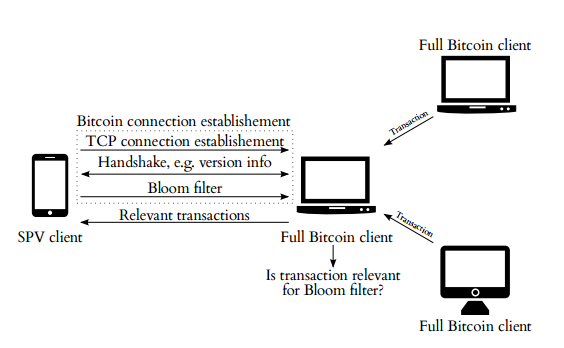
\includegraphics[width=0.7\linewidth]{./images/SPV}
	\caption{%
		ارتباط گره سبک با یک یا چند گره کامل در شبکهٔ همتا‌به‌همتای بیت‌کوین 
		\lr{\cite{Gervais2014}}
	}
	\label{fig:spv}
\end{figure}

	
\end{frame}

\subsection{فیلتر بلوم و آسیب‌پذیری‌ها}
\begin{frame}{فیلتر بلوم}
	\begin{figure}
		\centering
		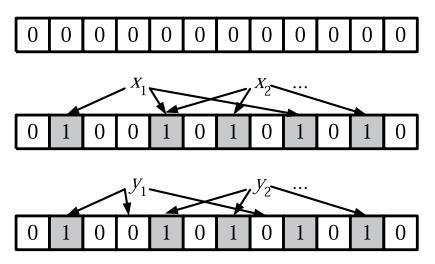
\includegraphics[width=0.7\linewidth]{images/BloomFilter}
		\caption{نمایش فیلتر بلوم
		\lr{\cite{Broder2004}}}
		\label{fig:bloomfilter}
	\end{figure}
\end{frame}

\begin{frame}{فیلتر بلوم در گره سبک (بیت‌کوین‌جی)}
	
	\begin{itemize}
		\item \lr{BIP 37}
		\item {%
			عناصر قرارداده شده:
			\begin{itemize}
				\item {
				چکیدهٔ تراکنش (\lr{TXID})، نبشته‌ها(\lr{Script}) در خروجی، \lr{COutPoint} در وردی، نبشته‌ها در ورودی}
			\end{itemize}
		}
		\item{$P_t=\%0.1$
		(نرخ خطای نوع دو)}
		\item{$M = m + 100 = 2N + 100$
		(ظرفیت)
			\begin{itemize}
				\item افزایش تدریجی اعضا
			\end{itemize}
		}
		\item{%
			قراردادن \lr{PubKey} و \lr{PubKeyHash}
			\begin{itemize}
				\item {باعث ایجاد آسیب‌پذیری
					 (\lr{\cite{Nick2015}})}
			\end{itemize}
		}
	\end{itemize}
\end{frame}

\begin{frame}{احتمال حدس آدرس‌های اصلی فیلتر بلوم}
	\framesubtitle{آسیب‌پذیری‌های فیلتر بلوم}
	$P_{h_{(j)}}$ 
	برابر است با احتمال حدس صحیح $j$ عنصر اصلی فیلتر بلوم \cite{Gervais2014}:
	\begin{table}
		
		\caption{%
			مقادیر 
			$P_{h_{(.)}}$
			با توجه به $N$
			($P_t=\%0.1$).
			\cite{Gervais2014}.
		}
		\label{table:P_h}
		\centering
		\begin{tabular}{|c|c|c|c|c|c|}
			\hline 
			\lr{$N$} & \lr{$1$} & \lr{$19$} & \lr{$49$}& \lr{$54$} & \lr{$8,999$}\\
			\hline
			\lr{$P_{h_{(1)}}$} & \lr{$1$} & \lr{$0.42$} & \lr{$0.0021$} & \lr{$0.14$} & \lr{$0.21$}\\
			%----
			\lr{$P_{h_{([N/2])}}$} & \lr{$-$} & \lr{$0.000026$} & \lr{$0$} & \lr{$0$} & \lr{$0$}\\
			%----
			\lr{$P_{h_{([N])}}$} & \lr{$1$} & \lr{$0$} & \lr{$0$} & \lr{$0$} & \lr{$0$}\\
			\hline
			
		\end{tabular}
		
	\end{table}
	افزایش این احتمال با در دست داشتن فیلتر‌های بلوم متعدد با عناصر مشترک
\end{frame}


\begin{frame}{عدم توجه به حاشاپذیری}
	\framesubtitle{آسیب‌پذیری‌های فیلتر بلوم}
	
	\begin{figure}
		\centering
		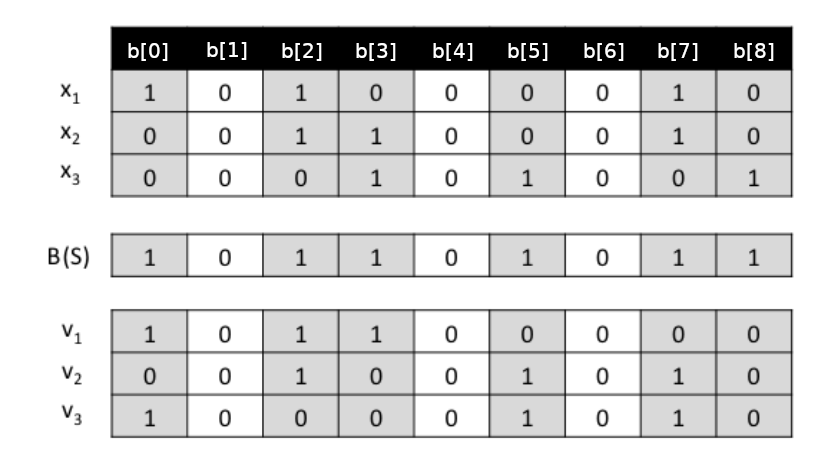
\includegraphics[width=0.7\linewidth]{images/gamma_deniability}
		\caption{%
			یک فیلتر بلوم با عناصر اصلی $\{x_1, x_2, x_3\}$ و عناصر پوششی $\{v_1, v_2, v_3\}$ \cite{Bianchi2012}.}
		\label{fig:gammadeniability}
	\end{figure}
	
\end{frame}

\begin{frame}{باقی آسیب‌پذیری‌ها}
	\framesubtitle{آسیب‌پذیری‌های فیلتر بلوم}
	\begin{enumerate}
		\item {%
		بار پردازشی بالا سمت گره کامل $\Leftarrow$ حملهٔ منع خدمت ($DoS$)} 
		\item {%
		عدم اتصال مداوم گره‌های سبک به شبکهٔ همتا‌به‌همتای بیت‌کوین
			\begin{itemize}
				\item{%
			بررسی ترکانش‌های منطبق شده با فیلتر بلوم که در همسایگی زمان درخواست گره سبک در زنجیرهٔ بلوکی ثبت شده‌اند.}
				\item{%
			مقایسهٔ بسامد درخواست کاربر سبک با بسامد تراکنش‌های منطبق شده.
			}
			\end{itemize}	
		\item {%
		تحلیل گراف تراکنش‌ها و حذف تراکنش‌های غیر مرتبط
		}
		\item {%
		حذف تراکنش‌هایی که شامل آدرسی ساخته شده قبل از \lr{BIP37} }
}
	\end{enumerate}
\end{frame}

\section{مروری بر کار‌های انجام شده\hfill}
\subsection{اصلاح رفتار کاربر سبک}
\begin{frame}{اصلاح رفتار کاربر سبک}
	\begin{itemize}
		\item {%
		قرار ندادن جفت مقدار \lr{PubKey} و \lr{PubKeyHash} در یک فیلتر بلوم.}
		\item {%
		استفاده از تمام ظرفیت فیلتر بلوم}
		\item {%
		ساخت فیلتر بلوم با آدرس‌هایی که تحت مالکیت گره سبک نیست.
		\begin{itemize}
			\item ساخت آدرس با توجه به فیلتر بلوم تولید شده
			\item بار پردازشی بالا سمت گره سبک
		\end{itemize}	
	}
		\item {%
		پرهیز از ایجاد فیلتر‌های بلوم متعدد با عناصر مشترک
		}
	\end{itemize}
	
	\begin{center}
		{\small \lr{\cite{Gervais2014}: \ Gervais et al., \textit{Proceedings of the 30th Annual Computer Security Applications Conference}}} 
	\end{center}
\end{frame}
\subsection{%
	معیار حاشاپذیری-$\gamma$}
\begin{frame}{%
		معیار حاشاپذیری-$\gamma$}
	
	محاسبهٔ $\gamma$ با توجه به فرمول زیر:
	
	\begin{equation}
	\gamma \left(B\right) \approx \left(1-exp\left(-\frac{N_vk}{n\left(1-e^{-km/n}\right)}\right)\right)^k
	\label{eq:gamma-deniability}
	\end{equation}
	
	\begin{itemize}
		\item $N_v=(N_u-m)\times P_f$
		\item استفاده از رگرسیون خطی برای تخمین $N_u$
	\end{itemize}
	\begin{center}
		{\small \lr{\cite{Kanemura2017}: \ Kanemura et al., \textit{2017 IEEE 28th Annual International Symposium on Personal, Indoor, and Mobile Radio Communications (PIMRC)}}}
	\end{center}
\end{frame}

\subsection{فیلتر کردن بلوک}

\begin{frame}{فیلتر کردن بلوک}
	\begin{itemize}
		\item{\lr{BIP 157, 158}}
		\item {%
		گره کامل به ازای هر بلوک یک «فیلتر بلوک» تولید می‌کند.}
		\item{%
		استفاده از روش کدگذاری گلومب-رایس برای فشرده سازی فیلتر}
		\item{%
		احتمال خطای نوع ۲ برابر $\frac{1}{M}$} است.
		\item{%
		حجم تخمینی برای یک فیلتر بلوک به ازای 
	$M = 784931$
و
	$P = 19$
کمتر از 
	$18$
کیلوبایت است.}
	\end{itemize}

	\begin{center}
	{\small \lr{\cite{Osuntokun2017}: \ Osuntokun et al., \textit{bips/bip-0157.mediawiki at master {\textperiodcentered} bitcoin/bips - Client Side Block Filtering}}}
	\end{center}

\end{frame}

\subsection{بازیابی اطلاعات خصوصی}
\begin{frame}{بازیابی اطلاعات خصوصی}
\begin{itemize}
	\item {%
	استفاده از روش ترکیبی \lr{IT-PIR} و \lr{C-PIR}}
	\item {%
	کاربر لازم است که سرایند زنجیرهٔ بلوکی و فایل‌های مانیفست را داشته باشد.}
	\item {%
	تقسیم‌بندی پایگاه داده به سه دستهٔ هفتگی، ماهانه و تمام مدت و ایجاد مانیفست برای هر کدام.
	\begin{itemize}
		\item {%
		حجم فایل مانیفست برای دستهٔ هفتگی، ماهانه و تمام-مدت به ترتیب $72$، ‌$218$ مگابایت و $3$ گیگابایت است.}
	\end{itemize}
	\item{%
	پیشنهاد خرد کردن دستهٔ تمام-مدت به چند زیر دستهٔ کوچک‌تر.}
}
\end{itemize}

\begin{center}
	{\small \lr{\cite{Qin2019}: \ Qin et al., \textit{2019 Crypto Valley Conference on Blockchain Technology, CVCBT 2019}}}
\end{center}
\end{frame}

\subsection{محیط اجرای قابل اعتماد}
\begin{frame}{محیط اجرای قابل اعتماد}
	\begin{itemize}
		\item {%
		استفاده از \lr{SGX}}
		\item{%
			ارائه دو روش
			\begin{enumerate}
				\item {%
				 پنجرهٔ پویش (\lr{Scanning Window})
			\begin{itemize}
				\item نرمالایز کردن اندازهٔ پاسخ و اطلاعات جست‌وجو شده
				\item {%
				جلوگیری از حملهٔ زمانی $\leftarrow$ سربار پردازشی زیاد ($73$ ثانیه برای پردازش $100$ بلوک)}
			\end{itemize}	 
		 }
			 	\item {%
			 	 و پایگاه دادهٔ ناآگاهانه (\lr{‫‪Oblivious‬‬ ‫‪Database‬‬})
		 	 \begin{itemize}
		 	 	\item {%
		 	 	بهره‌گیری از $ORAM$}
	 	 		\item{%
	 	 		بدون نیاز به اثبات مرکل}
	 	 \end{itemize}}
			\end{enumerate}
		}
	\end{itemize}

\begin{center}
	{\small \lr{\cite{Matetic2019}: \ Matetic et al., \textit{Proceedings of the 28th USENIX Security Symposium}}}
\end{center}
\end{frame}


\section{ارائهٔ روش\hfill}
\subsection{ایدهٔ پروتکل، فروض و تعاریف}
\begin{frame}{ایدهٔ پروتکل}
	\begin{multicols}{2}
		\begin{itemize}
			\item{%
				ایده از مقالهٔ \lr{ \cite{Niu2015}}
			}
			\item{%
			آدرس‌های پوششی دارای احتمال پرسمان یکسانی با آدرس اصلی باشند.
		$\leftarrow$
	افزایش آنتروپی درخواست.}
		\end{itemize}
	\columnbreak
		\begin{figure}
			\centering
			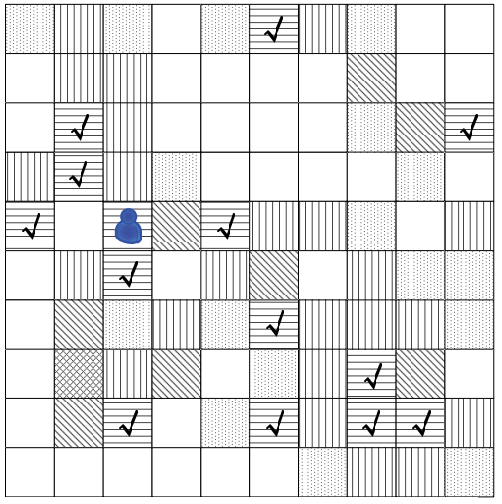
\includegraphics[width=0.7\linewidth]{images/LBS_Kanonymity}
			\label{fig:lbskanonymity}
		\end{figure}
	\end{multicols}

\begin{center}
	{\small \lr{\cite{Niu2015}: \ Niu et al., \textit{Proceedings - IEEE INFOCOM 2015}}}
\end{center}
\end{frame}

\begin{frame}{فرض و تعاریف}
	\begin{block}{فرض}
		‫احتمال درخواست اطلاعات مربوط به هر آدرس $a_n$، به شرطی که مربوط به یک گره کامل نباشد، متناسب است با احتمال استفاده از آن آدرس در شبکهٔ بیت‌کوین.
	\end{block}

\begin{equation}
Pr\{{a_n}\} = 
\begin{cases}
0, & \text{if}\ a_n \in A_{f_j},\ \ \forall_{j} : 1<j<W \\
Pr\{{a_{l_{ic}}}\}, & \text{if}\ a_n = a_{l_{ic}} \in A_{l_i},\ \ \forall_{i,c} : 1<i<M,\  1<c<C_{l_i}
\end{cases} \label{eq:3}
\end{equation}


\begin{equation}
Pr\{{a_n}\} \propto p(a_n) \triangleq \frac{|T_{a_n}|}{\sum_{m=1}^{N}|T_{a_m}|}; \forall i \  a_n \in A_{l_i}  \label{eq:4}
\end{equation}

\end{frame}


\subsection{ملزومات پروتکل}
\begin{frame}{ملاحظات مستقل از سازوکار پروتکل}
	\framesubtitle{ملزومات پروتکل}
	کلیات:
	\begin{itemize}
		\item {حفظ حریم خصوصی کاربر سبک}
		\item {بار محاسباتی و پهنای باند مصرفی پایین}
		\item {عدم الزام به اضافه کردن تجهیزات سخت‌افزاری یا نرم‌افزاری غیر معمول به گره کامل}
		\item {
			امکان سادهٔ ارائهٔ خدمات مبتنی بر روش ارائه شده $\leftarrow$ جلوگیری از متمرکز شدن شبکه.}
		\item {نیاز به اعتماد به دیگر گره‌های شبکه تا حد امکان پایین باشد.}
	\end{itemize}
\end{frame}

\begin{frame}{ملزومات پروتکل}
	ملاحظات در انتخاب آدرس‌های هم احتمال
	\begin{itemize}
		\item کاربر سبک امکان محاسبهٔ بسامد دخ‌داد همهٔ آدرس‌ها در زنجیرهٔ بلوکی را ندارد
		\item {%
			 درخواست مستقیم آدرس‌های هم احتمال با یک آدرس مشخص از یک گره کامل $\leftarrow$ نیازمند اعتماد و نقض حریم خصوصی}
		 \item {%
		 باید اطلاعات اضافه‌ٔ در خواست داده شده حداقل شود.}
		 \item {%
		 تغییر مداوم آدرس‌های پوششی باعث به خطر افتادن حریم خصوصی کاربر سبک می‌شود.}
	\end{itemize}
\end{frame}

\subsection{ساختار پروتکل}
\begin{frame}{محاسبهٔ مستقل از دیگر آدرس‌ها}
	\begin{itemize}
		\item {%
		هر گره سبک باید تعداد تراکنش‌های مرتبط با خود را ذخیره نماید.}
		\item {%
			برای هر آدرس $a_n$ یک امتیاز به صورت زیر محاسبه می‌شود
		} 
	\end{itemize}

\begin{equation}
s_{a_n}^{t_0} = \beta NT_{a_n}^{t_0} + (1-\beta) s_{a_n}^{t_0-1}
\label{eq:6}
\end{equation}

\begin{itemize}
	\item {%
	هر دوره زمانی قابل تنظیم است. در این پیاده‌سازی مقدار آن برابر یک روز یا $144$ بلوک در نظر گرفته شده است.}
\end{itemize}

\end{frame}

\begin{frame}{امتیاز آدرس‌های بیت‌کوین}
	\begin{figure}[t]
		\centering
		\includegraphics[width=0.7\linewidth]{/home/taghi/Projects/Bitcoin_Address_Extractor/Analysis/Log2_scale}
		\caption[امتیاز آدرس‌های بیت‌کوین در مقیاس لگاریتمی]{امتیاز آدرس‌های بیت‌کوین در مقیاس لگاریتمی از ۲۶ ژوئن ۲۰۱۹ الی ۰۲ دسامبر ۲۰۱۹}
		\label{fig:log2scale}
	\end{figure}
\end{frame}

\begin{frame}{محاسبه‌ٔ آفلاین در سمت کاربر سبک}
	\begin{itemize}
		\item{%
			در طراحی انجام شده، گره‌های سبک لازم است اطلاعات زیر را ذخیره داشته باشد:
	\begin{itemize}
		\item سرایند زنجیرهٔ بلوکی
		\item تمام تراکنش‌های مرتبط با خودش و این که در کدام بلوک‌ها قرار گرفته‌اند
\end{itemize}	}
		\item {%
		امتیاز به صورت آفلاین و بدون نیاز به ارسال اطلاعات اضافی قابل محاسبه است.}
		\item {
			اگر کاربر سبک سابقه تراکنش‌هایش را نداشت، می‌تواند با آزمون و خطا تکه‌های مختلف را امتحان نماید.
			}
		\item{%
		قراردادن آدرس‌ها با ترتیب الفبایی درون تکه‌ها}
	\end{itemize}
\end{frame}

\subsection{پیاده‌سازی و شبیه‌سازی}

\begin{frame}{ابزارهای پیاده‌سازی شده}
	\framesubtitle{پیاده‌سازی و شبیه‌سازی}
	\begin{itemize}
		\item {%
			راه‌اندازی در کنار نرم‌افزار هستهٔ بیت‌کوین
		\begin{itemize}
			\item عدم استفاده از واسط‌های برنامه‌نویسی
			\item تجزیهٔ مستقیم فایل‌های \lr{blk.dat}
			\item امکان تجزیهٔ انواع نبشته‌ها
		\end{itemize}}
		\item {%
		استفاده از پایگاه دادهٔ ردیس
		\begin{itemize}
			\item {%
			نیاز به $36$ گیگ حافظهٔ دائمی}
		\end{itemize}
}
	\end{itemize}
\end{frame}

\begin{frame}{تغییر آدرس‌ها در میان تکه‌ها}
	\begin{figure}[h]
		\centering
		\includegraphics[width=0.7\linewidth]{/home/taghi/Projects/Bitcoin_Address_Extractor/Analysis/changed}
		\caption{%
			جابه‌جایی آدرس‌ها در میان تکه‌های مختلف از ۲۶ ژوئن ۲۰۱۹ الی ۰۲ دسامبر ۲۰۱۹. ($\beta=0.3$)
		}
		\label{fig:changed}
	\end{figure}
\end{frame}

\begin{frame}{به روزرسانی و هم‌گام‌سازی}
	\begin{itemize}
		\item {%
		با حذف آدرس‌های با موجودی صفر، زمان محاسبهٔ امتیاز آدرس‌ها از $25$ دقیقه به $2$ دقیقا کاهش پیدا می‌کند.}
		\item {%
		در همگام‌سازی اولیهٔ یک گره کامل تازه‌ اضافه شده، می‌توان تنها امتیاز آدرس‌هایی که در روز‌های مورد بررسی استفاده شده‌اند را بررسی نمود.}
	\end{itemize}
\end{frame}

\begin{frame}{زمان به روز‌رسانی وضعیت‌ها در حالت هم‌گام‌سازی}
\begin{figure}[h!]
	\centering
	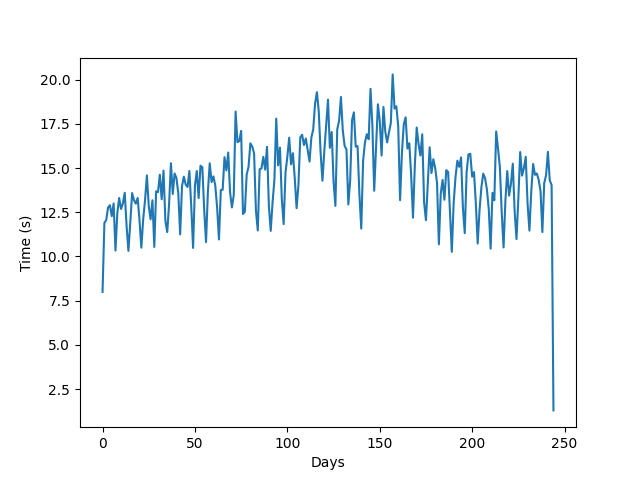
\includegraphics[width=0.7\linewidth]{../tehran-thesis/image/time}
	\caption[زمان‌ به روز رسانی وضعیت امتیاز‌ها برای هر روز]{ زمان‌ به روز رسانی امتیاز‌ها برای هر روز از  $19$ ژانویه $2019$ الی $21$ سپتامبر $2019$.}
		\label{fig:time}
	\end{figure}
\end{frame}

\subsection{بحث و مقایسه}
\begin{frame}{امنیت}
	\framesubtitle{بحث و مقایسه}
	\begin{itemize}
		\item امکان تعیین آدرس‌های پوششی به صورت هوشمندانه و به مقدار دلخواه
		\item استقلال بین درخواست‌های متفاوت کاربر سبک
		\item مقاوم در برابر تحلیل بسامد
		\item عدم نیاز به تجهیزات سخت‌افزاری و نرم‌افزاری پیچیده
		\item{%
			 امکان سادهٔ راه‌اندازی گره‌های کامل ارائه دهندهٔ این خدمت $\leftarrow$ تمرکز کمتر شبکه}
	\end{itemize}
\end{frame}

\begin{frame}{پهنای باند مصرفی و پردازش سمت کاربر}
	\framesubtitle{بحث و مقایسه}
	پهنای باند مصرفی:
	\begin{itemize}
		\item قابل تنظیم، شامل تراکنش‌های اصلی به علاوهٔ تراکنش‌های پوششی و اثبات مرکل آن
	\end{itemize}

	پردازش سمت گره کامل:
	\begin{itemize}
		\item پردازش سنگینی در سمت گره کامل وجود ندارد
	\end{itemize}
\end{frame}

\section{کارهای آینده\hfill}
\begin{frame}{کارهای آینده}
	\begin{itemize}
		\item صحت‌سنجی فرض انجام شده با استفاده از آزمایش
		\item تعیین پارامتر بهینهٔ $\beta$
	\end{itemize}
\end{frame}

\begin{frame}[allowframebreaks, plain]{مراجع}
%	\lr{
%	\begin{thebibliography}
%		\bibitem[Dijkstra, 1982]
%		E.~Dijkstra.
%		\newblock Smoothsort, an alternative for sorting in situ.
%		\newblock {\em Science of Computer Programming}, 1(3):223--233, 1982.\\
%		\bibitem[Gervais, 2016] 
%		A. ~Gervais.
%		\newblock {On The Privacy Provisions of Bloom Filters in Lightweight Bitcoin Clients.}
%		\newblock {\em ACM International Conference Proceeding Series}\\
%	\end{thebibliography}	
%}
	\bibliographystyle{alpha}
	\lr{%
		{\small \bibliography{ref.bib}}}
	
\end{frame}


\end{document}